% !TeX program = xelatex
% Build: python build.py
\documentclass[aspectratio=169,10pt]{beamer}
\usepackage[UTF8,fontset=fandol]{ctex}
\usepackage{amsmath,amssymb,booktabs,array,tabularx,etoolbox}
\usepackage{tikz,pgfplots}
\usetikzlibrary{arrows.meta,positioning,calc,fit}
\pgfplotsset{compat=1.18}
\usefonttheme{professionalfonts}
\setbeamertemplate{navigation symbols}{}
\setbeamertemplate{headline}{}
\setbeamertemplate{itemize item}{\small\textbullet}
\setbeamertemplate{itemize subitem}{\tiny\textbullet}
\definecolor{Ink}{HTML}{18333B}
\definecolor{Teal}{HTML}{087F83}
\definecolor{Amber}{HTML}{B66B24}
\definecolor{Muted}{HTML}{52646A}
\definecolor{Paper}{HTML}{F6F8F7}
\definecolor{Line}{HTML}{C7D8D7}
\setbeamercolor{normal text}{fg=Ink,bg=white}
\setbeamercolor{structure}{fg=Teal}
\setbeamercolor{frametitle}{fg=Ink}
\setbeamercolor{title}{fg=Ink}
\setbeamercolor{block title}{fg=Teal,bg=white}
\setbeamercolor{block body}{fg=Ink,bg=white}
\setbeamerfont{title}{size=\LARGE,series=\bfseries}
\setbeamerfont{frametitle}{size=\large,series=\bfseries}
\setbeamerfont{block title}{size=\normalsize,series=\bfseries}
\setbeamersize{text margin left=8mm,text margin right=8mm}
\setbeamertemplate{frametitle}{\vspace{3mm}\insertframetitle\par\vspace{2mm}}
\setbeamertemplate{footline}{\hfill\textcolor{Muted}{\scriptsize\ifnum\value{framenumber}>26 备份\ \number\numexpr\value{framenumber}-26\relax\else\insertframenumber\,/\,26\fi}\hspace{6mm}\vspace{3mm}}
\setlength{\parskip}{4pt}
\newcommand{\src}[1]{\vfill{\fontsize{6.7}{8}\selectfont\color{Muted}#1}\par}
\newcommand{\lead}[1]{{\color{Teal}\large\bfseries #1}\par\medskip}
\newcommand{\term}[1]{\textcolor{Teal}{\textbf{#1}}}
\newcommand{\warn}[1]{\textcolor{Amber}{#1}}
\newcolumntype{Y}{>{\raggedright\arraybackslash}X}
\AfterEndEnvironment{tabularx}{\par}
\tikzset{box/.style={draw=Line,fill=Paper,minimum height=9mm,align=center,inner sep=5pt,font=\small},
arr/.style={-{Latex[length=2mm]},thick,draw=Teal},
labeltext/.style={font=\scriptsize,text=Muted,align=center}}
\title{大模型基础设施与 Agent 工程}
\subtitle{面试项目介绍}
\author{陶壮\quad Zhuang Tao}
\date{2026 年 11 月}
\hypersetup{pdftitle={大模型基础设施与 Agent 工程：面试项目介绍},pdfauthor={Zhuang Tao},pdfsubject={Interview Project Portfolio},pdfkeywords={MoE,load balancing,simulation,agent,harness}}

\begin{document}
\begin{frame}[plain]
\vspace{11mm}
{\color{Teal}\small PROJECTS\quad /\quad SYSTEMS\quad /\quad ENGINEERING}\par
\vspace{5mm}
{\usebeamerfont{title}\inserttitle\par}
\vspace{4mm}
{\large\insertsubtitle\par}
\vspace{11mm}
{\normalsize\insertauthor}\par
{\small\color{Muted}\insertdate}
\end{frame}

\begin{frame}{项目经历覆盖推理系统、数据平台、服务网关与 Agent 执行}
\renewcommand{\arraystretch}{1.55}
\begin{tabularx}{\textwidth}{@{}p{3.2cm}YY@{}}
\toprule 大项目 / 项目 & 平台解决的问题 & 我的主要工作 \\
\midrule
\shortstack[l]{OmniInfer\\Omni-EPLB} & 大模型推理加速；专家均衡能力的框架集成与 SDK 交付 & 专家均衡、运行时、工具测试、框架与模型适配 \\
企业数据工程平台 & 数据资产、处理产线与生产任务的统一管理 & DataHub 扩展、注册 SDK、身份权限、Data Agent \\
Omni-ELB / LiteLLM & 应用到多套模型后端的统一调用入口 & 协作路由设计、状态刷新、指标修复 \\
路由 simulator & 在服务主链路之外研究和验证调度策略 & 插件接入、事件引擎、服务后端与实验工具 \\
编码 Agent 平台 & 多会话 Agent 的任务组织、执行观察与结果交付 & Delm 双 worker 适配、Harness² 接入与可靠执行 \\
\bottomrule
\end{tabularx}
\src{下面按“项目背景 → 整体架构 → 我的职责与技术 → 代表问题”介绍；不同平台分别建设，不预设为一套系统。}
\end{frame}

\section{推理系统：OmniInfer 与 Omni-EPLB}
\begin{frame}{OmniInfer、OmniPlacement 与 Omni-EPLB 分别是框架、能力与 SDK}
\renewcommand{\arraystretch}{1.7}
\begin{tabularx}{\textwidth}{@{}p{3cm}YY@{}}
\toprule 名称 & 项目定位 & 与我工作的关系 \\
\midrule
OmniInfer & 总体推理加速框架，组合注意力、专家均衡与 P/D 调度能力 & 我主要参与专家均衡，同时参与框架与模型接入修复 \\
OmniPlacement & MoE 专家排布与负载均衡能力；历史上集成于 OmniInfer & 核心算法工程、运行时、Pattern 工具、配置与测试 \\
Omni-EPLB & 相关均衡能力独立演进的 Python/C++ SDK，核心包为 \texttt{omni\_placement} & 延续相关能力及接入工程；独立通信 context 是可核验的后续贡献 \\
\bottomrule
\end{tabularx}
\medskip
\term{总体框架中的能力集成 → 独立 SDK 交付与持续适配。}
\src{SDK 独立不代表替代全部 OmniInfer；同源能力迁移不重复统计为新的原创算法。}
\end{frame}

\begin{frame}{OmniInfer 组合引擎计算优化与服务调度，面向大模型推理}
\lead{背景：MoE 热点、长上下文计算和预填充/解码阶段需求不同}
{\small MoE（混合专家）每个 token 只调用部分专家；P/D 分别指预填充与解码。}\par
\begin{center}
\begin{tikzpicture}[node distance=6mm]
\node[box,text width=2.0cm] (a) {客户端请求};
\node[box,text width=2.7cm,right=of a] (b) {OmniProxy\\请求生命周期与 P/D 调度};
\node[box,text width=3.5cm,right=of b] (c) {推理引擎与并列加速能力\\OmniAttn\\\mbox{\term{OmniPlacement}}};
\node[box,text width=2.2cm,right=of c] (d) {设备运行时\\算子与通信};
\draw[arr] (a)--(b);\draw[arr] (b)--(c);\draw[arr] (c)--(d);
\end{tikzpicture}
\end{center}
\begin{itemize}
\item \term{OmniAttn}：稀疏注意力与 KV 缓存模式优化；\term{OmniPlacement}：专家排布与运行时均衡。
\item \term{OmniProxy}：在服务层组织请求及预填充/解码资源，兼顾缓存与负载。
\item 论文实现以 vLLM 为底座；仓库另有 SGLang 等接入与模型适配。
\end{itemize}
\src{以上是团队框架整体。我的主要模块是专家均衡与相关适配，不将 OmniAttn/OmniProxy 的全部设计归为个人工作。}
\end{frame}

\begin{frame}{我在 OmniInfer 中以专家均衡为主，也参与框架与模型接入}
\renewcommand{\arraystretch}{1.5}
\begin{tabularx}{\textwidth}{@{}p{2.4cm}Yp{3cm}@{}}
\toprule 工作域 & 我的具体工作 & 主要技术 \\
\midrule
算法工程 & 副本分配、受约束布局、动态候选与更新门槛 & C++ / Python、堆与贪心、负载建模 \\
运行时执行 & 激活采集、批量传输、权重与映射更新、通信 context 延续 & PyTorch、C++ 扩展、ACL / HCCL \\
工具与质量 & Pattern 流水线、CLI/YAML、配置模板及 Python/C++ 测试 & NumPy、构建工具、单元测试 \\
框架/模型适配 & vLLM/SGLang 接入、共享/zero expert、模型部署配置和局部兼容修复 & 框架 hooks、张量形状与状态、启动配置 \\
\bottomrule
\end{tabularx}
\src{外围协作包括 Qwen3-Next P/D 配置、causal\_conv 状态形状和 MLA dummy-run 调用修复。它们按适配/局部修复介绍，不扩写为整个注意力或调度组件的设计。}
\end{frame}

\begin{frame}{Omni-EPLB 将专家均衡封装为可接入推理框架的 SDK}
\lead{项目目标：把布局、统计和更新接口从总体框架中独立交付}
\begin{center}
\begin{tikzpicture}[node distance=6mm]
\node[box,text width=2.5cm] (a) {推理框架 hooks\\模型与插件适配};
\node[box,text width=2.5cm,right=of a] (b) {Python Planner\\配置、映射与张量接口};
\node[box,text width=2.5cm,right=of b] (c) {pybind11 / C++\\统计、优化与权重更新};
\node[box,text width=2.5cm,right=of c] (d) {设备与通信\\ACL / HCCL};
\draw[arr] (a)--(b);\draw[arr] (b)--(c);\draw[arr] (c)--(d);
\end{tikzpicture}
\end{center}
\begin{itemize}
\item \term{输入契约}：合法 Pattern、模型层与专家信息、并行规模及权重地址。
\item \term{运行接口}：逻辑到物理映射、激活采集、候选决策和安全点更新。
\item \term{交付资产}：Python 包/C++ 扩展、配置、Pattern 工具，以及 CPU mock/条件设备测试。
\end{itemize}
\src{这是进程内 SDK 接入，不是独立 HTTP 路由服务。当前实现包含 Ascend 工具链依赖；个人贡献与 SDK 的全部团队能力分别说明。}
\end{frame}

\begin{frame}{MoE 的稀疏激活把单轮时延推向最忙的设备}
\begin{columns}[T]
\begin{column}{.47\textwidth}
\lead{专家数量相同，工作量仍可能悬殊}
\begin{itemize}
\item 路由到逻辑专家的频率随输入变化。
\item 热门专家副本过少，会集中计算压力。
\item 复制权重消耗容量；布局还受通信与唯一性约束。
\end{itemize}
\medskip
\[T_{\mathrm{layer}}\approx\max_d T_d+T_{\mathrm{comm}}\]
\end{column}
\begin{column}{.48\textwidth}
\begin{tikzpicture}
\begin{axis}[width=\linewidth,height=4.5cm,ybar,bar width=9mm,ymin=0,ymax=20,
symbolic x coords={A,B,C,D},xtick=data,ylabel={示意工作量},ytick={0,8,16},
axis lines=left,tick label style={font=\small},label style={font=\small},enlarge x limits=.2]
\addplot[fill=Teal,draw=none] coordinates {(A,18)(B,6)(C,5)(D,7)};
\end{axis}
\end{tikzpicture}
\end{column}
\end{columns}
\src{图中数据仅解释拖尾机制，不是硬件测试。OmniPlacement 是 OmniInfer 团队系统中的专家排布与均衡能力。}
\end{frame}

\begin{frame}{动态均衡把采集、候选决策与权重更新连成闭环}
\begin{center}
\begin{tikzpicture}[node distance=6mm]
\node[box,text width=2.6cm] (a) {物理槽激活采集\\还原逻辑专家负载};
\node[box,text width=2.6cm,right=of a] (b) {候选布局搜索\\触发与改善门槛};
\node[box,text width=2.6cm,right=of b] (c) {迁移指令与批次\\通信、缓冲与同步};
\node[box,text width=2.6cm,right=of c] (d) {安全点切换映射\\重建统计语义};
\draw[arr] (a)--(b);\draw[arr] (b)--(c);\draw[arr] (c)--(d);
\draw[arr] (d.south)--++(0,-.6)-|(a.south);
\end{tikzpicture}
\end{center}
\medskip
\begin{itemize}
\item 统计必须对应当前布局，多个副本要汇总到同一逻辑专家。
\item 当前不均衡达到触发阈值、候选改善超过裕度后才更新。
\item 运行时采用布局代理收益；热点持续期和复制时间的成本判据在模拟中另行建模。
\end{itemize}
\src{运行时链条按项目能力介绍；本人重点贡献包括优化器、工具链、批量传输、测试和多模型适配。}
\end{frame}

\begin{frame}{框架适配保留逻辑专家选择，并转换物理执行位置}
\begin{center}
\begin{tikzpicture}[node distance=6mm]
\node[box,text width=2.5cm] (a) {Gate 输出\\逻辑专家 ID 与分数};
\node[box,text width=2.5cm,right=of a] (b) {Planner / selector\\查询物理副本};
\node[box,text width=2.5cm,right=of b] (c) {副本轮转与特殊掩码\\保留 \mbox{token} 与分数};
\node[box,text width=2.5cm,right=of c] (d) {物理专家 ID\\交给原推理执行路径};
\draw[arr] (a)--(b);\draw[arr] (b)--(c);\draw[arr] (c)--(d);
\end{tikzpicture}
\end{center}
\medskip
\renewcommand{\arraystretch}{1.45}
\begin{tabularx}{\textwidth}{@{}p{4cm}Y@{}}
\toprule 接口或适配点 & 实现职责 \\
\midrule
\texttt{plan()} & 使用传入的当前层映射，将逻辑专家转换为物理位置 \\
\texttt{record\_activation()} & 采集物理位置上的激活，供统计与候选决策使用 \\
\texttt{place\_experts()} & 在主路径安全点应用已就绪权重与映射更新 \\
模型差异 & 层索引、稠密前缀、共享 / zero expert 和 Pattern 维度分别适配 \\
\bottomrule
\end{tabularx}
\src{本人参与接口、配置、多模型与特殊专家适配。这里不改变 Gate 的逻辑选择，不推定所有框架和模型均已完成同等实测。}
\end{frame}

\begin{frame}{推理方向的交付包括框架模块、独立 SDK 延续与工具测试}
\renewcommand{\arraystretch}{1.55}
\begin{tabularx}{\textwidth}{@{}p{2.8cm}YY@{}}
\toprule 交付 & 已形成的能力或证据 & 面试中可展开的技术问题 \\
\midrule
框架集成 & OmniInfer 中的专家均衡实现、模型配置与局部兼容修复 & 怎样把算法接入实际执行路径 \\
SDK 演进 & 独立 Omni-EPLB 延续，含通信 context 相关贡献 & Python/C++ 边界、设备状态与通信生命周期 \\
工具与质量 & 采集、Pattern、配置、单元与条件硬件测试入口 & 数据口径、约束检查、失败定位 \\
论文与复现 & OmniInfer 论文共同作者；公开合成模型与原始记录 & 如何区分组件效果、团队系统结果和模型假设 \\
\bottomrule
\end{tabularx}
\src{系统论文：\url{https://arxiv.org/abs/2511.22481}。合成结果和算法细节放在技术备份中，均保留测试条件与收益边界。}
\end{frame}

\section{企业数据工程平台}
\begin{frame}{数据工程平台管理数据资产、处理产线与生产任务}
\lead{面向数据工程师和资产治理人员，解决生产过程与数据来源的追溯问题}
\begin{center}
\begin{tikzpicture}[node distance=7mm]
\node[box,text width=2.6cm] (a) {统一门户\\资产、任务与结果};
\node[box,text width=3.3cm,right=of a] (b) {团队业务服务\\资产 / 产线版本 / 任务管理};
\node[box,text width=2.8cm,right=of b] (c) {Runtime\\按版本执行产线};
\node[box,text width=5.2cm,below=9mm of b] (d) {元数据底座：DataHub、事件与索引\\直接注册 API 与异步事件分别接入};
\draw[arr] (a)--(b);\draw[arr] (b)--(c);\draw[arr] (b)--(d);\draw[arr] (c.south)|-(d.east);
\end{tikzpicture}
\end{center}
\begin{itemize}
\item DataHub 是开源元数据底座，提供实体、搜索、Schema 和血缘等基础能力。
\item 我重点负责元数据接入、企业治理与智能交互，平台的任务执行等模块由团队协作建设。
\end{itemize}
\src{本页是平台功能架构，省略内部系统标识、实际部署与业务规模；同步注册与异步事件不是单一串行链路。}
\end{frame}

\begin{frame}{我在数据平台中横跨注册服务、身份权限、前端与 Agent}
\renewcommand{\arraystretch}{1.5}
\begin{tabularx}{\textwidth}{@{}p{2.7cm}Yp{3.4cm}@{}}
\toprule 本人模块 & 实现内容 & 技术栈 \\
\midrule
Extensions / 注册 SDK & 分层重构、统一 API、URN/Aspect、注册与修改约束 & Python、FastAPI、\mbox{Pydantic}、DataHub SDK \\
企业身份与授权 & SSO/准入、领域与角色策略、用户凭证衔接 & Java / GMS、GraphQL、Play \\
平台页面 & 资产操作、注册、授权与凭证等界面适配 & React、TypeScript、HTTP API \\
Data Agent & 元数据工具编排、流式交互、实体链接与回归支持 & Python、SSE、MCP 工具、元数据 API \\
\bottomrule
\end{tabularx}
\src{上游 DataHub 与团队任务/Runtime 能力不归为个人开发。下面以注册 SDK 和 Data Agent 两条实际链路说明设计。}
\end{frame}

\begin{frame}{注册 SDK 用分层接口连接资产建模、读写和验证}
\begin{center}
\begin{tikzpicture}[node distance=6mm]
\node[box,text width=2.5cm] (a) {HTTP API\\或进程内直接调用};
\node[box,text width=2.5cm,right=of a] (b) {MetadataService\\身份、依赖与注册编排};
\node[box,text width=2.5cm,right=of b] (c) {Entity / Aspect\\URN 与变更提案构造};
\node[box,text width=2.5cm,right=of c] (d) {查询与发布适配\\GraphQL / ES / Emitter};
\draw[arr] (a)--(b);\draw[arr] (b)--(c);\draw[arr] (c)--(d);
\end{tikzpicture}
\end{center}
\medskip
\renewcommand{\arraystretch}{1.45}
\begin{tabularx}{\textwidth}{@{}p{2.5cm}Y@{}}
\toprule 工程决策 & 作用与边界 \\
\midrule
计算与 I/O 分离 & URN / Aspect 可独立校验；搜索走 ES，存在性和精确读取走 GraphQL \\
注册约束集中 & 服务端注入主体、检查域与依赖；同 URN 的注册用进程内锁协调 \\
发布与查询分开 & REST / Kafka 按路径选择；发送后轮询确认可查询，超时显式返回 \\
\bottomrule
\end{tabularx}
\src{本人负责扩展重构、API/SDK 与注册约束。发布成功不等于索引已可查询；进程内锁和轮询确认不构成跨副本事务。}
\end{frame}

\begin{frame}{元数据 Agent 用工具结果建立可追溯的回答}
\begin{center}
\begin{tikzpicture}[node distance=7mm]
\node[box,text width=2.2cm] (q) {用户问题};
\node[box,text width=2.6cm,right=of q] (a) {Agent 编排\\调用元数据工具};
\node[box,text width=3.4cm,right=of a] (t) {搜索 / 实体 / 血缘\\Schema / Profile / 注册};
\draw[arr] (q)--(a);\draw[arr] (a)--(t);
\node[box,text width=3.4cm,below=7mm of t] (r) {结构化元数据与实体引用};
\node[box,text width=2.6cm,left=of r] (ans) {回答与实体链接};
\draw[arr] (t)--(r);\draw[arr] (r)--(ans);
\end{tikzpicture}
\end{center}
\begin{itemize}
\item 工具访问已有元数据和权限服务，语言模型负责交互与编排。
\item 返回实体链接，用户可以检查来源并继续浏览资产。
\item 本人实现工具接入、结果实体链接、配置和回归支持。
\end{itemize}
\src{注册工具设权限门禁并传递操作主体；读取工具的逐用户细粒度授权仍需进一步验证。}
\end{frame}

\section{推理网关与离线仿真}
\begin{frame}{Omni-ELB 的 LiteLLM 网关为应用连接多套模型服务后端}
\lead{目标：统一调用入口，并管理健康候选、路由、状态与观测}
\begin{center}
\begin{tikzpicture}[node distance=6mm]
\node[box,text width=2.4cm] (a) {应用 / Agent};
\node[box,text width=2.7cm,right=of a] (b) {入口代理\\转发与连接管理};
\node[box,text width=2.8cm,right=of b] (c) {LiteLLM 网关\\统一 API 与凭证\\模型配置与路由};
\node[box,text width=2.4cm,right=of c] (d) {多套模型服务\\后端内部执行 P/D};
\draw[arr] (a)--(b);\draw[arr] (b)--(c);\draw[arr] (c)--(d);
\node[labeltext,below=8mm of c,text width=7cm] {侧向依赖：Redis 状态、Prometheus 观测、PostgreSQL；\\控制链路负责状态刷新与服务管理};
\end{tikzpicture}
\end{center}
\begin{itemize}
\item LiteLLM 提供上游网关框架，团队在其基础上集成策略、部署与运维能力。
\item 我主要参与健康候选生成后的集群选择，以及路由依赖的状态和指标链路。
\end{itemize}
\src{项目还有其他数据面/控制面实现方向；本页只介绍本人参与的 LiteLLM 路径，不推定所有实现串联部署。}
\end{frame}

\begin{frame}{我共同设计会话与负载路由，并独立修复状态与计量链路}
\renewcommand{\arraystretch}{1.55}
\begin{tabularx}{\textwidth}{@{}p{2.6cm}YY@{}}
\toprule 本人工作 & 关键设计或修复 & 用到的技术 \\
\midrule
协作路由算法 & 保持健康会话；新会话进入低负载候选；状态缺失时保留回退路径 & Python / asyncio、LiteLLM hook、Redis、稳定散列 \\
独立状态刷新 & 自动发现部署、聚合 P 侧压力、稳定 ID 关联和漏刷诊断 & HTTP API、Prometheus、批量状态读写 \\
重复计数修复 & 日志过滤与监控回调分离，保留唯一计量路径 & callback 调用链、监控 counter、回归用例设计 \\
\bottomrule
\end{tabularx}
\medskip
代表取舍：会话复用保护缓存机会，负载感知缓解热点；两者都依赖准确且及时的状态。
\src{路由是与同事共同设计；刷新和重复计数修复有个人直接提交证据。不将整体路由结果拆成单次修复的独立收益。}
\end{frame}

\begin{frame}{部署发现与稳定标识连接减少负载状态的静默漏刷}
\begin{center}
\begin{tikzpicture}[node distance=5mm]
\node[box,text width=2.5cm] (a) {\texttt{/model/info}\\发现模型组与部署 ID};
\node[box,text width=2.5cm,right=of a] (b) {Prometheus 聚合\\P 侧 running + waiting};
\node[box,text width=2.5cm,right=of b] (c) {部署 ID 精确关联\\写 \mbox{Redis} 负载键};
\node[box,text width=2.5cm,right=of c] (d) {需重选时批量 MGET\\保持路由路径简洁};
\draw[arr] (a)--(b);\draw[arr] (b)--(c);\draw[arr] (c)--(d);
\end{tikzpicture}
\end{center}
\medskip
\renewcommand{\arraystretch}{1.45}
\begin{tabularx}{\textwidth}{@{}p{3.2cm}Y@{}}
\toprule 异常或边界 & 具体处理 \\
\midrule
running / waiting 单边存在 & 按实例聚合后外连接，保留单边记录，再按集群求和 \\
部署未匹配监控标签 & 显式列出漏刷项，区分缺部署与疑似命名脱节 \\
配置发现接口不可用 & 可显式采用配置降级，并在日志注明实际来源 \\
\bottomrule
\end{tabularx}
\src{本人直接实现独立刷新链路。P 侧请求数是代理负载；刷新时间与状态年龄判断仍需补强，不把它等同剩余 token 工作量。}
\end{frame}

\begin{frame}{Simulator 是网关项目的离线路由实验工具}
\lead{背景：策略改动需要固定输入、可控状态和可替换的服务耗时假设}
\begin{center}
\begin{tikzpicture}[node distance=6mm]
\node[box,text width=2.4cm] (a) {合成 / 脱敏轨迹};
\node[box,text width=2.8cm,right=of a] (b) {离散事件引擎\\派发、完成与在途状态};
\node[box,text width=2.6cm,right=of b] (c) {真实插件直接挂载\\独立状态适配};
\node[box,text width=2.6cm,right=of c] (d) {服务耗时后端\\指标与校准报告};
\draw[arr] (a)--(b);\draw[arr] (b)--(c);\draw[arr] (c)--(d);
\end{tikzpicture}
\end{center}
\begin{itemize}
\item \term{我的工作}：模块架构、采集/校准、插件调用、事件引擎、经验后端和实验编排。
\item \term{主要技术}：Python、异步插件接口、事件最小堆、Redis 适配、CSV/JSON 与 CLI。
\item \term{用途}：回归真实路由逻辑、检查状态恢复、筛选策略和研究假设敏感性。
\end{itemize}
\src{它位于生产请求主链路之外。llm\_repro 是另一套公开合成模型；服务 simulator 不逐 token 仿真真实 P/D 内核。}
\end{frame}

\begin{frame}{统一数据契约使采集、插件与服务后端可以分别替换}
\renewcommand{\arraystretch}{1.55}
\begin{tabularx}{\textwidth}{@{}p{2.6cm}YY@{}}
\toprule 接口边界 & 输入与输出 & 工程检查点 \\
\midrule
TraceRecord & 请求 ID、到达、token、E2E、模型组；落点 / TTFT 可选 & 采集时校验字段，保留路由键的完整语义 \\
路由插件 & 请求、健康候选与状态适配；返回目标部署 & 直接加载原模块，用会话探针检查选点分支 \\
服务 Backend & 请求规模、当前在途与命中近似；返回 E2E / TTFT & 参数化与经验后端共享调用接口，耗时单位明确 \\
运行归档 & 运行元数据、种子列表与汇总指标 & 记录代码提交；逐种子明细、完整拟合参数与输入哈希仍需补齐 \\
\bottomrule
\end{tabularx}
\medskip
\term{插件导入、路由真正生效、服务模型有效，是三个可以分别诊断的问题。}
\src{本人实现模块拆分、Backend 解耦、采集与插件调用修正。契约兼容不意味着任意插件的外部依赖已经被完整仿真。}
\end{frame}

\section{编码 Agent 平台}
\begin{frame}{编码 Agent 平台把任务、实时执行和项目结果集中管理}
\lead{面向个人开发者与小团队，让多个自主 Agent 在项目工作区执行任务}
\renewcommand{\arraystretch}{1.65}
\begin{tabularx}{\textwidth}{@{}p{2.8cm}Y@{}}
\toprule 平台整体能力 & 用户获得的工作方式 \\
\midrule
任务组织 & 提交任务、共享计划、会话派发与运行队列；失败后暂停等待处理 \\
执行观察 & 多会话并行，实时展示模型与工具事件，重新连接后读取历史 \\
项目交付 & 文件浏览与编辑、项目记忆、执行摘要和日志持久化 \\
\bottomrule
\end{tabularx}
\medskip
\term{我的两块工作：Delm 双 worker 协作适配，以及 Harness² 配置调优接入。}
\src{上述 UI、队列和平台底座按团队整体介绍。前端使用原生 JavaScript 与 CodeMirror；不将整个平台归为个人实现。}
\end{frame}

\begin{frame}{我的模块位于 Agent 运行时内部，以及配置调优的执行入口}
\begin{center}
\begin{tikzpicture}[node distance=6mm]
\node[box,text width=2.4cm] (a) {Web 界面\\任务与计划\\聊天与文件};
\node[box,text width=2.6cm,right=of a] (b) {Node 服务\\HTTP / WebSocket\\会话与运行队列};
\node[box,text width=3cm,right=of b] (c) {Agent 运行时\\单 Agent / \term{Delm 双 worker}\\模型 SDK 与 MCP};
\node[box,text width=2.4cm,right=of c] (d) {项目工作区\\代码、测试、产物};
\draw[arr] (a)--(b);\draw[arr] (b)--(c);\draw[arr] (c)--(d);
\node[box,draw=Teal,text width=4.5cm,below=9mm of b] (e) {\term{Harness² 执行适配}\\Python 调优器 → Node runner};
\draw[arr] (e.east)-|(c.south);
\end{tikzpicture}
\end{center}
\begin{itemize}
\item 平台底座使用 Node.js / Express / WebSocket，保存计划、会话与 JSON/JSONL 事件。
\item 我负责的适配让协作运行时与调优器共用实际执行路径，并回收轨迹与候选产物。
\end{itemize}
\src{高亮处为本人主要模块。Delm 协作语义与 Harness² 搜索方法有上游来源；本人重点在运行时工程与可靠执行。}
\end{frame}

\begin{frame}{DELM 适配把双 worker 协作组织成可追溯的看板状态}
\begin{center}
\begin{tikzpicture}[node distance=8mm]
\node[box,text width=2.4cm] (a) {worker A\\独立执行上下文};
\node[box,text width=2.6cm,right=of a] (b) {MCP 工具边界\\绑定 actor 身份};
\node[box,text width=2.7cm,right=of b] (c) {追加式事件日志\\派生看板视图};
\node[box,text width=2.4cm,below=8mm of a] (d) {worker B\\独立执行上下文};
\draw[arr] (a)--node[above,labeltext]{actor A}(b);\draw[arr] (d.east)-|node[pos=.25,below,labeltext]{actor B}(b.south);\draw[arr] (b)--(c);
\end{tikzpicture}
\end{center}
\begin{itemize}
\item 每个 worker 同时最多认领一项未完成任务（claim），显式记录状态。
\item 进程内事件唤醒等待者，减少对看板的盲目轮询。
\item 本人完成相关 JavaScript 运行时适配、工具桥接与会话组织。
\end{itemize}
\src{DELM 沿用上游框架称谓，不扩展缩写；看板协议来源与本地适配分别归因，不宣称个人原创整个协议。}
\end{frame}

\begin{frame}{Harness² 接入让提示、工具与协作规则成为可执行的配置变体}
\lead{Harness 是执行配置组合：提示、规则、技能、工具指南和协作约定}
\begin{center}
\begin{tikzpicture}[node distance=6mm]
\node[box,text width=2.5cm] (a) {上游调优器\\提出并组织配置变体};
\node[box,draw=Teal,text width=2.5cm,right=of a] (b) {本人执行桥接\\Python / Node 契约};
\node[box,draw=Teal,text width=2.5cm,right=of b] (c) {配置实际物化\\单 / 双 worker 运行};
\node[box,text width=2.5cm,right=of c] (d) {轨迹与可读产物\\候选比较、人工验收};
\draw[arr] (a)--(b);\draw[arr] (b)--(c);\draw[arr] (c)--(d);
\end{tikzpicture}
\end{center}
\begin{itemize}
\item \term{我实现的链路}：输入准备、配置接线、CLI/JSON 契约、轨迹转换与结果回收。
\item \term{我解决的可靠性问题}：并发运行互相覆盖、输入遗漏、已有输入文件（seed）修改被漏报、长任务停滞。
\item \term{技术栈}：Python、Node.js、文件系统、内容哈希、JSONL、单元回归。
\end{itemize}
\src{真实执行是系统能力；本轮离线测试不等于真实模型任务成功率提升。上游搜索的候选范围与完整验证结果在备份页说明。}
\end{frame}

\begin{frame}{可靠交付需要分开判断运行、产物与任务正确性}
\renewcommand{\arraystretch}{1.6}
\begin{tabularx}{\textwidth}{@{}lYY@{}}
\toprule 机制 & 本人实现或修正 & 避免的问题 \\
\midrule
输入 staging & 任务文本哈希、输入额度与存储根配置 & 不同任务错误复用输入或遗漏必要文件 \\
运行作用域 & 用户/会话命名空间、重跑工作区重建 & 并发覆盖和上次产物残留 \\
产物识别 & 比较 seed 内容，保留新增或已改文件 & 修改原文件却被误判为无交付 \\
停滞处理 & 逐 worker 观察、提醒与失败窗口 & 活跃 worker 掩盖静默同伴 \\
\bottomrule
\end{tabularx}
\medskip
\term{正常退出、存在工具活动、有候选产物、通过任务验收，是四个不同判断。}
\src{输入哈希并非完整项目内容寻址；运行目录存在也不证明 Agent 已执行。采纳配置与回收工作产物分别处理。}
\end{frame}

\section{技术总结}
\begin{frame}{我的技术栈集中在推理运行时、平台后端与 Agent 执行工程}
\renewcommand{\arraystretch}{1.55}
\begin{tabularx}{\textwidth}{@{}p{2.6cm}YY@{}}
\toprule 技术面 & 实际使用的技术 & 解决过的具体问题 \\
\midrule
推理运行时 & C++、Python、PyTorch、pybind11、ACL/HCCL & 专家映射、激活统计、权重迁移和安全更新 \\
平台与治理后端 & FastAPI、Pydantic、Java、GraphQL、Play & 注册 SDK、身份权限、API 和前端凭证衔接 \\
服务与状态 & Redis、Prometheus、异步 hook、HTTP API & 会话路由、负载刷新、回退和计量正确性 \\
Agent 与实验 & Node.js、MCP、事件日志、Python 仿真、内容哈希 & 协作状态机、执行契约、产物检测与结果回收 \\
\bottomrule
\end{tabularx}
\src{前端实践包括 React/TypeScript 的数据平台适配；编码 Agent 平台的前端底座另为原生 JavaScript。技术标签均对应实际参与模块。}
\end{frame}

\begin{frame}{可进一步展开的代表性问题}
\renewcommand{\arraystretch}{1.8}
\begin{tabularx}{\textwidth}{@{}p{4.7cm}Y@{}}
\toprule 项目问题 & 我可以展开的设计与取舍 \\
\midrule
怎样把专家均衡算法接入推理框架 & 副本/布局约束、Python/C++ 接口、通信批次、映射安全生效 \\
怎样让平台状态成为可靠的决策输入 & 稳定标识、注册与权限语义、状态刷新、计量修复和降级 \\
怎样交付可检查的 Agent 运行结果 & 看板协作、输入与运行隔离、产物内容比较、采纳与回收 \\
\bottomrule
\end{tabularx}
\medskip
\term{技术备份包含算法细节、实验口径、运行协议和测试结果，可按问题展开。}
\src{公开资料与原创复现：\url{https://github.com/taostronger/llm-mock-1}。后续页为技术备份。}
\end{frame}

\appendix
\section{技术备份}
\begin{frame}{备份：副本分配先降低单副本压力，再处理设备组合}
\begin{columns}[T]
\begin{column}{.51\textwidth}
\lead{固定预算的整数资源分配}
\[\min_{r}\ \max_e\frac{a_e}{r_e}\]
\[1\le r_e\le u_e,\quad r_e\in\mathbb Z,\quad\sum_e r_e\le E+B\]
\begin{itemize}
\item $a_e$：固定窗口内专家工作量。
\item $r_e$：副本数；$B$：额外副本预算。
\item 每次给当前 $a_e/r_e$ 最大的专家增加副本。
\end{itemize}
\end{column}
\begin{column}{.44\textwidth}
\renewcommand{\arraystretch}{1.5}
\begin{tabular}{@{}lrrr@{}}
\toprule 专家 & $a_e$ & 初始 $r_e$ & 分配后 $r_e$\\\midrule
1 & 12 & 1 & 2\\
2 & 8 & 1 & 2\\
3 & 4 & 1 & 1\\
4 & 4 & 1 & 1\\\bottomrule
\end{tabular}
\par\medskip
最大单副本压力：$12\rightarrow6$。
\par\smallskip
\warn{这一步的最优性不等于设备布局全局最优。}
\end{column}
\end{columns}
\src{条件：固定非负工作量、等成本副本、均匀分担与整数上限。堆分配时间 $O(E+B\log E)$。例子为流程示意。}
\end{frame}

\begin{frame}{备份：设备放置同时满足容量、同卡唯一性与负载目标}
\begin{columns}[T]
\begin{column}{.48\textwidth}
\[x_{de}\in\{0,1\},\quad \sum_d x_{de}=r_e\]
\[\sum_e x_{de}\le C_d,\qquad L_d=\sum_e x_{de}\frac{a_e}{r_e}\]
\[\min_x\max_d L_d\]
副本按压力降序放置，在可行设备中选择较低负载目标。
\par\medskip
拓扑重排进一步分散主机间热点，采用具体分组规则。
\end{column}
\begin{column}{.46\textwidth}
\begin{tikzpicture}[node distance=6mm]
\node[box,minimum width=4.8cm] (a) {设备 A：$e_1(6)+e_2(4)+e_3(4)$};
\node[box,minimum width=4.8cm,below=of a] (b) {设备 B：$e_1(6)+e_2(4)+e_4(4)$};
\node[labeltext,below=of b,text width=4.8cm] {每设备 3 个槽位；同一专家不重复落在同一设备。\quad $L_A=L_B=14$};
\end{tikzpicture}
\par\medskip
\warn{贪心可能因顺序而构造失败；可行性和负载质量分别检查。}
\end{column}
\end{columns}
\src{示例沿用上一页工作量；原静态函数不是任意拓扑的最优求解器。公开复现中的最大流回退仅保证合法布局。}
\end{frame}

\begin{frame}{备份：迁移按冲突拆批，并在权重就绪后更新映射}
\begin{columns}[T]
\begin{column}{.46\textwidth}
\lead{控制面产生差异指令}
\begin{enumerate}
\item 比较当前布局与目标布局。
\item 将新增、移除与传输指令分组。
\item 拆分存在 rank 冲突的批次。
\end{enumerate}
\end{column}
\begin{column}{.49\textwidth}
\lead{数据面控制可见状态}
\begin{enumerate}
\item 后台通信写入缓冲并同步完成状态。
\item 主线程在安全点把就绪数据复制到设备。
\item 更新变更层的 selector，清理标志并切换统计口径。
\end{enumerate}
\end{column}
\end{columns}
\medskip
\begin{center}
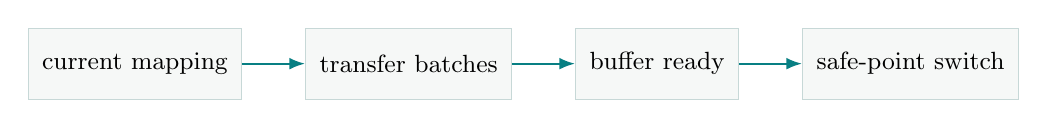
\begin{tikzpicture}[node distance=8mm]
\node[box] (a) {current mapping};\node[box,right=of a] (b) {transfer batches};
\node[box,right=of b] (c) {buffer ready};\node[box,right=of c] (d) {safe-point switch};
\draw[arr] (a)--(b);\draw[arr] (b)--(c);\draw[arr] (c)--(d);
\end{tikzpicture}
\end{center}
\src{OmniPlacement / Omni-EPLB 运行时设计摘要。未把整套框架、所有通信机制或系统性能归为个人独立成果。}
\end{frame}

\begin{frame}{备份：Pattern 工具链把激活记录转换为可检查的部署文件}
\begin{center}
\begin{tikzpicture}[node distance=5mm]
\node[box,text width=2.45cm] (a) {日志 / 文本\\采集窗口与 rank};
\node[box,text width=2.45cm,right=of a] (b) {激活工作量 CSV\\层与专家记录};
\node[box,text width=2.45cm,right=of b] (c) {副本与布局生成\\Pattern 文件};
\node[box,text width=2.45cm,right=of c] (d) {覆盖与槽位检查\\热图和负载对照};
\draw[arr] (a)--(b);\draw[arr] (b)--(c);\draw[arr] (c)--(d);
\end{tikzpicture}
\end{center}
\medskip
\renewcommand{\arraystretch}{1.45}
\begin{tabularx}{\textwidth}{@{}p{2.5cm}Y@{}}
\toprule 工程环节 & 具体实现与检查对象 \\
\midrule
输入契约 & 区分 prefill / decode、统计步区间、层数与专家数，核对采集位置与专家编号的关系 \\
输出产物 & rank $\times$ layer $\times$ expert 的部署文件，以及基线/候选负载 CSV 和可视化 \\
接入检查 & 工具检查专家覆盖与各 rank 数量一致性；Planner 启动时检查并行规模匹配 \\
\bottomrule
\end{tabularx}
\src{本人工作包括 Pattern 流水线、CLI/YAML、适配和测试。覆盖检查不等于所有约束都已独立验证；完整交付宜同时保存采集窗口与配置。}
\end{frame}

\begin{frame}{备份：合成模拟中，热点变化决定动态更新的价值}
\begin{columns}[c]
\begin{column}{.66\textwidth}
\begin{tikzpicture}
\begin{axis}[width=.97\linewidth,height=5cm,ybar,bar width=5pt,ymin=0,xmin=-.6,xmax=4.6,
xtick=data,xticklabels={稳态,突变,交替,均匀,高复制成本},
ylabel={单层服务时延 / ms},enlarge x limits=false,axis lines=left,
tick label style={font=\scriptsize},label style={font=\small},
legend style={at={(.5,1.05)},anchor=south,legend columns=3,draw=none,font=\scriptsize}]
\addplot[fill=Muted!45,draw=none] table[x=index,y=uniform,col sep=comma]{data/eplb.csv};
\addplot[fill=Teal,draw=none] table[x=index,y=static,col sep=comma]{data/eplb.csv};
\addplot[fill=Amber,draw=none] table[x=index,y=dynamic,col sep=comma]{data/eplb.csv};
\legend{均匀副本,静态,动态}
\end{axis}
\end{tikzpicture}
\end{column}
\begin{column}{.31\textwidth}
\term{动态相对静态}
\par\medskip
稳态偏斜：$0.0\%$\par
热点突变：$-42.1\%$\par
高复制成本：$-33.6\%$
\par\medskip
过去窗口预测；更新代价计入同步复制。
\par\medskip
\warn{不是 GPU/NPU 或完整模型测速。}
\end{column}
\end{columns}
\src{来源：results/reference/eplb\_aggregate.csv；3 个固定种子均值，360 步，逻辑激活与显式时间模型。}
\end{frame}

\begin{frame}{备份：算法一优先保持会话，并为新会话选择低负载候选}
\textcolor{Muted}{\small 下表为合成复现中的统一策略口径。}\par\medskip
\renewcommand{\arraystretch}{1.8}
\begin{tabularx}{\textwidth}{@{}p{3.4cm}@{\hspace{5mm}}Y@{}}
\toprule 请求分支 & 路由动作 \\
\midrule
已有健康映射 & 保持原后端，延续缓存复用机会 \\
新建亲和会话 & 从最低负载的 $k=\max(1,\lceil0.1N\rceil)$ 个候选中选择 \\
无亲和要求 & 按请求形态进入最小负载或稳定散列路径 \\
\bottomrule
\end{tabularx}
\medskip
\begin{columns}[T]
\begin{column}{.46\textwidth}\term{优点}\par 机制直接，兼顾会话稳定性与新流量分散。\end{column}
\begin{column}{.49\textwidth}\warn{边界}\par 已有会话遇到拥堵时，保持映射可能继续累积等待。\end{column}
\end{columns}
\src{0.1 是该算法的候选比例，不是理论最优常数。合成模拟的统一 P/D 计数协议见 docs/MODEL.md。}
\end{frame}

\begin{frame}{备份：算法二用等待收益与缓存损失比较决定是否切换}
\lead{已有会话从 A 切换到 B 的简化判据}
\[\underbrace{\widehat W_A-\widehat W_B}_{\text{预计减少的等待}}
>\underbrace{1.2\,\widehat\theta_A\bar n/v}_{\text{原端缓存收益的时间估计}}\]
\begin{columns}[T]
\begin{column}{.49\textwidth}
\begin{itemize}
\item $\widehat W_i$：可观测状态下的预计等待。
\item $\widehat\theta_A$：原端历史 token 复用比例。
\item $\bar n/v$：平均输入的预填充时间尺度。
\end{itemize}
\end{column}
\begin{column}{.45\textwidth}
\begin{itemize}
\item 两侧单位均为时间。
\item 统计缺失、相等时保持会话。
\item 决策前切换；不迁移在执行的请求或缓存。
\end{itemize}
\end{column}
\end{columns}
\src{这是理论分析与模拟策略。模拟不读取 B 的真实缓存，执行时仍计算实际命中；1.2 的裕度不构成预测误差保证。}
\end{frame}

\begin{frame}{备份：缓存容量与状态延迟会改变切换策略的收益方向}
\begin{columns}[c]
\begin{column}{.66\textwidth}
\begin{tikzpicture}
\begin{axis}[width=.97\linewidth,height=5.1cm,xbar,bar width=9pt,ymin=-.5,ymax=4.5,
ytick=data,yticklabels={稳态8后端,热点转移,流量突发,小缓存,观测延迟},
xlabel={算法二相对算法一的平均 TTFT 变化 / \%},
xmin=-25,xmax=32,axis lines=left,y dir=reverse,
tick label style={font=\scriptsize},label style={font=\small},grid=major,grid style={Line!45}]
\addplot[fill=Teal,draw=none] table[y=index,x=change_pct,col sep=comma]{data/routing.csv};
\end{axis}
\end{tikzpicture}
\end{column}
\begin{column}{.31\textwidth}
\term{同一策略存在收益与退化}
\par\medskip
突发：$-18.31\%$\par
小缓存：$+18.14\%$\par
观测延迟：$+26.15\%$
\par\medskip
负值为变快，正值为变慢。目标端缓存与预测误差不能忽略。
\end{column}
\end{columns}
\src{来源：results/reference/routing\_aggregate.csv；3 固定种子、合成请求、显式 P/KV/D 时间模型；非真实服务性能。}
\end{frame}

\begin{frame}{备份：批量读写、变化集同步与内存适配降低状态访问开销}
\begin{columns}[T]
\begin{column}{.48\textwidth}
\lead{保留相同状态口径，减少重复工作}
\begin{enumerate}
\item 将多键状态读写合并为批量操作。
\item 在完成与派发后跟踪变化集群，减少全量重复同步。
\item 在适用场景用进程内存储承接高频状态调用。
\end{enumerate}
\end{column}
\begin{column}{.47\textwidth}
\lead{检查优化后的接口行为}
\begin{itemize}
\item 比对同步后的在途计数和插件落点。
\item 分开记录模拟时间与真实执行墙钟。
\item 单列真实 Redis 与内存模式的语义覆盖。
\end{itemize}
\end{column}
\end{columns}
\medskip
\renewcommand{\arraystretch}{1.4}
\begin{tabularx}{\textwidth}{@{}p{2.5cm}Y@{}}
\toprule 模式 & 当前边界 \\
\midrule
真实 Redis & 键过期受墙钟影响，需要核对快速模拟时钟与 TTL 的关系 \\
内存适配 & 未完整实现 TTL / Lua / 原子语义，适合匹配接口的受控扫描 \\
\bottomrule
\end{tabularx}
\src{这些是已实现的开销优化路径；本次未新增性能测速，不给出未经测量的加速倍数或生产收益。}
\end{frame}

\begin{frame}{备份：开环回放与闭环容量回答不同的实验问题}
\begin{center}
\begin{tikzpicture}[node distance=4mm]
\node[box,text width=1.65cm] (a) {请求派发};
\node[box,text width=1.65cm,right=of a] (b) {插件选点\\在途加一};
\node[box,text width=1.65cm,right=of b] (c) {后端返回\\E2E / TTFT};
\node[box,text width=1.65cm,right=of c] (d) {完成事件\\进入最小堆};
\node[box,text width=1.65cm,right=of d] (e) {时钟推进\\释放在途};
\draw[arr] (a)--(b);\draw[arr] (b)--(c);\draw[arr] (c)--(d);\draw[arr] (d)--(e);
\end{tikzpicture}
\end{center}
\medskip
\renewcommand{\arraystretch}{1.5}
\begin{tabularx}{\textwidth}{@{}lYY@{}}
\toprule 模式 & 到达方式 & 适用问题 \\
\midrule
开环回放 & 保留输入到达过程 & 给定流量下的状态和策略行为 \\
闭环容量 & 固定并发水位，完成后补位 & 指定水位与模型下的完成率 \\
\bottomrule
\end{tabularx}
\src{服务后端返回请求级耗时，未逐 token 模拟 P/D、KV 链路或连续批处理；这些细化机制属于 llm\_repro 参考模型。}
\end{frame}

\begin{frame}{备份：条件回放与反事实预测需要不同的验证证据}
\renewcommand{\arraystretch}{1.65}
\begin{tabularx}{\textwidth}{@{}lYY@{}}
\toprule
模式 & 已知信息与用途 & 能够支持的结论 \\
\midrule
条件回放 & 注入真实落点及观测时序；检查原路径 & 给定条件下的决策与记录一致性 \\
经验后端 & 用观测样本或拟合关系描述执行成本 & 已覆盖负载范围内的条件估计 \\
反事实策略对照 & 重算落点、在途与会话命中近似 & 需要独立验证新分布下的计时与排序 \\
\bottomrule
\end{tabularx}
\medskip
\warn{将真实时延带回回放，可以核对链路；它不能证明新策略的时延预测准确。}
\src{共享同一个后端模型也不自动保证策略排序正确：策略改变会反过来改变会话命中、在途和并发分布。}
\end{frame}

\begin{frame}{备份：日志、claim 与文件哈希共同约束协作一致性}
\renewcommand{\arraystretch}{1.65}
\begin{tabularx}{\textwidth}{@{}lYY@{}}
\toprule 机制 & 约束 & 工程意义 \\
\midrule
事件追加 & 状态由日志归约为视图 & 可以追踪任务认领和状态变化 \\
单 worker 单 claim & 认领与完成显式执行 & 避免一个 worker 同时占据多项工作 \\
actor 绑定 & 工具调用的主体由会话绑定 & 不依赖模型自行填对身份 \\
文件 apply 校验 & 用 SHA-256 检查预期基础内容 & 发现已变化的文件，拒绝冲突写入 \\
\bottomrule
\end{tabularx}
\medskip
\warn{进程内事件与文件冲突检查不等于跨进程事务或任意并发条件下的形式化保证。}
\src{哈希保护仅覆盖 board.apply；worker 直接编辑共享文件仍可能冲突。公开报告不附源项目代码与配置。}
\end{frame}

\begin{frame}{备份：Harness2 将执行框架变体纳入真实 rollout 的搜索循环}
\begin{center}
\begin{tikzpicture}[node distance=6mm]
\node[box,text width=2.5cm] (a) {$k$ 个基线运行\\收集执行证据};
\node[box,text width=2.5cm,right=of a] (b) {$2k$ 个 INV/DOM\\提案与运行};
\node[box,text width=2.5cm,right=of b] (c) {$k$ 个 AGG 合成\\配置与 rollout};
\node[box,text width=2.5cm,right=of c] (d) {只对 AGG 产物盲选\\再独立验收};
\draw[arr] (a)--(b);\draw[arr] (b)--(c);\draw[arr] (c)--(d);
\draw[arr] (d.south)--++(0,-.6)-|(a.south);
\end{tikzpicture}
\end{center}
\medskip
\begin{itemize}
\item 被优化的是执行系统的可变部分，而不只是一段静态提示词。
\item 并行模式最终选择池不包含基线或中间变体，没有内建弃选。
\item 本人负责 Harness2 运行时适配、可靠执行和 Agent 接线；搜索方法源于上游。
\end{itemize}
\src{图示为上游并行搜索流程；顺序模式另有候选链。选中候选不证明优于基线，需要独立任务测试。}
\end{frame}

\begin{frame}{备份：版本化 runner 将候选配置落到真实执行和可读结果}
\renewcommand{\arraystretch}{1.55}
\begin{tabularx}{\textwidth}{@{}p{2.4cm}Y@{}}
\toprule 工程接口 & 已实现的接线与产物 \\
\midrule
调用输入 & 任务目录、harness 目录、run ID、模式和超时；运行标识进入路径前校验 \\
配置物化 & 合并系统提示与规则，映射技能/工具指南/子代理，注入两 worker 启动提示和看板指导 \\
进程协议 & stdout 只返回单行 JSON，stderr 承载进度；原始事件转换为统一轨迹文本 \\
结果目录 & \texttt{trajectory.txt}、\texttt{events*.jsonl}（双 worker 分别记录）、\texttt{workspace/}、\texttt{meta.json} 与 runner 报告 \\
\bottomrule
\end{tabularx}
\medskip
执行状态、工具活动、候选产物分别保留；无法获得的成本写为空值，不用零值代替。
\src{本人负责执行桥接、配置接线和轨迹转换；上游提供搜索组织方法。runner 契约通过不等于模型任务已通过。}
\end{frame}

\begin{frame}{备份：配置采纳与任务产物回收分开，支持审阅和文件级恢复}
\begin{center}
\begin{tikzpicture}[node distance=7mm]
\node[box,text width=2.4cm] (a) {diff\\检查实际配置差异};
\node[box,text width=2.4cm,right=of a] (b) {snapshot\\保存目标文件原状};
\node[box,text width=2.4cm,right=of b] (c) {adopt\\写入选中配置};
\node[box,text width=2.4cm,right=of c] (d) {rollback\\恢复配置文件};
\draw[arr] (a)--(b);\draw[arr] (b)--(c);\draw[arr] (c)--node[above,labeltext]{可选}(d);
\end{tikzpicture}
\end{center}
\medskip
\begin{columns}[T]
\begin{column}{.48\textwidth}
\lead{配置操作}
\begin{itemize}
\item 采纳前比较物化后的实际映射。
\item 恢复旧内容，删除本次新增的配置文件。
\end{itemize}
\end{column}
\begin{column}{.47\textwidth}
\lead{独立回收 workspace}
\begin{itemize}
\item 提取新增或内容改变的任务文件。
\item 排除配置和记账文件；过滤项列出清单。
\end{itemize}
\end{column}
\end{columns}
\src{这是本人承担的结果管理与可靠交付工程。rollback 仅恢复采纳涉及的配置文件，不回滚 Agent 的全部项目修改，也不提供整项目事务。}
\end{frame}

\begin{frame}{备份：离线回归已覆盖核心机制，完整集成仍有明确缺口}
\renewcommand{\arraystretch}{1.6}
\begin{tabularx}{\textwidth}{@{}lYY@{}}
\toprule 验证对象 & 本轮实际结果 & 可以支持的结论 \\
\midrule
Board 单元测试 & 13/13 通过 & 看板关键状态与操作符合用例 \\
Harness2 JavaScript 测试 & 三套合计 58/58 通过 & 配置物化、runner dry-run 契约与轨迹渲染 \\
Python 全量发现 & 84 项：58 通过、9 失败、12 错误、5 跳过 & 旧任务接口和 seed fixture 与当前实现存在差异 \\
会话编排单元测试 & 所需 Agent SDK 缺失，加载终止 & 此项未执行；真实模型端到端实验另需开展 \\
\bottomrule
\end{tabularx}
\medskip
\warn{通过单元测试不等于多任务成功率提升；不宣称完整测试全绿。}
\src{基于已提交版本的独立快照执行；未将源工作区未提交变更作为结论依据。详见 docs/delm-harness2-technical-report.md。}
\end{frame}

\begin{frame}{备份：单副本子问题的性质不能外推到设备最优}
\begin{itemize}
\item 给定阈值 $t>0$，专家 $e$ 至少需要 $\lceil a_e/t\rceil$ 个副本，并满足 $1\le r_e\le u_e$。
\item 因此阈值可行性由各专家最低副本数、上限和总预算共同决定。
\item 给当前最大 $a_e/r_e$ 增加副本，求解固定等成本模型下的单副本瓶颈。
\item 设备目标 $\max_d\sum_e x_{de}a_e/r_e$ 还包含组合与容量限制；需单独求解。
\end{itemize}
\medskip
\renewcommand{\arraystretch}{1.4}
\begin{tabularx}{\textwidth}{@{}lY@{}}
\toprule 阶段 & 时间复杂度 \\
\midrule
副本分配 & $O(E+B\log E)$，heapify 加 B 次堆更新 \\
贪心放置 & $O(M\log M+MN+NE)$，$M=\sum_e r_e$ \\
\bottomrule
\end{tabularx}
\src{均匀分流、固定工作量、等成本是性质前提。放置空间含 $N\times E$ 映射矩阵，不是仅 $O(E)$。}
\end{frame}

\begin{frame}{备份：资料与复现入口}
\small
\begin{enumerate}
\item OmniInfer 团队论文：\emph{System-Wide Acceleration Techniques for Optimizing LLM Serving Throughput and Latency}.\par
\url{https://arxiv.org/abs/2511.22481}
\item Omni-EPLB 公开项目与原静态函数来源：\par
\url{https://gitee.com/omniai/omni-eplb}
\item 合成实验、固定参数与逐请求记录：\par
\url{https://github.com/taostronger/llm-mock-1}
\item 本仓库文档：\texttt{docs/MODEL.md}、\texttt{docs/ALGORITHMS\_SCENARIOS\_REPORT.md}。
\item 新增专题：\texttt{docs/simulator-technical-report.md}、\par
\texttt{docs/delm-harness2-technical-report.md}。
\item Agent 方法来源：上游 Delm 协作语义、上游 Harness² 搜索框架（Apache-2.0）；本文介绍运行时适配，不分发其代码。
\end{enumerate}
\src{本演示稿只包含原创概述、通用机制和公开合成结果；未分发 Agent 源项目代码、内部轨迹或部署配置。}
\end{frame}

\end{document}
